\documentclass[final]{beamer}

% ====================
% Packages
% ====================

\usepackage[T1]{fontenc}
\usepackage[utf8]{inputenc}
\usepackage{lmodern}
\usepackage[size=custom, width=122,height=91, scale=1.9]{beamerposter}
\usetheme{Berlin}
\usecolortheme{default}
\usepackage{graphicx}
\usepackage{booktabs}
\usepackage{tikz}
\usepackage{pgfplots}
\pgfplotsset{compat=1.14}
\usepackage{anyfontsize}
\usepackage{hyperref}
\usepackage{ragged2e}
\justifying

% ====================
% Lengths
% ====================

\newlength{\sepwidth}
\newlength{\colwidth}
\setlength{\sepwidth}{0.025\paperwidth}
\setlength{\colwidth}{0.3\paperwidth}

\newcommand{\separatorcolumn}{\begin{column}{\sepwidth}\end{column}}

% ====================
% PSU Color Palette
% ====================

\usepackage[x11names]{xcolor}
\definecolor{psugreen}{RGB}{33,57,33}
\definecolor{psulightgreen}{RGB}{109,141,36}
\definecolor{psugray}{RGB}{204,204,204}
\definecolor{psubluegray}{RGB}{66,91,111}
\definecolor{psuwhite}{RGB}{255,255,255}

\setbeamercolor{normal text}{fg=black, bg=white}
\setbeamercolor{frametitle}{fg=psuwhite,bg=psugreen}
\setbeamercolor{block title}{bg=psulightgreen, fg=psuwhite}
\setbeamercolor{block body}{bg=white, fg=black}
\setbeamercolor{caption name}{fg=psugreen}
\setbeamercolor{title}{fg=psuwhite, bg=psulightgreen}
\setbeamerfont{title}{size=\large}
\setbeamercolor{subtitle}{fg=psugreen, bg=white}

\setbeamertemplate{footline}{}


% ====================
% Title Configuration
% ====================

\title{Codefest Presentation}
\author{Tucker X Mastin}
\institute[shortinst]{Department of Electrical and Computer Engineering, Portland State University}
\date{}

% Fix title bar color
\setbeamertemplate{headline}{
  \vspace*{2cm} 
  \leavevmode
  \begin{beamercolorbox}[wd=\paperwidth,ht=4ex,dp=2ex,center]{frametitle}
    \usebeamerfont{title}\insertshorttitle
  \end{beamercolorbox}
  \vspace{1.5ex}
  \begin{beamercolorbox}[wd=\paperwidth,ht=2.5ex,dp=1ex,center]{subtitle}
    \usebeamerfont{subtitle}\insertauthor \hspace{1em} $\vert$ \insertinstitute
  \end{beamercolorbox}
}

% ====================
% Begin Document
% ====================

\begin{document}


\begin{frame}[t]


\vspace{1cm}

\begin{columns}[t]

\separatorcolumn

\begin{column}{\colwidth}

\begin{block}{What are you trying to do?}
I am building an analog model of a Leaky Integrate-and-Fire (LIF) spiking neuron, with the goal of assembling it into a Liquid State Machine (LSM) - a biologically-inspired recurrent neural network that processes temporal input data. In this architecture, the internal dynamics are untrained and only the readout layer is trained, making it an ideal candidate for analog acceleration.
\end{block}

\begin{block}{Visualizations}
\centering
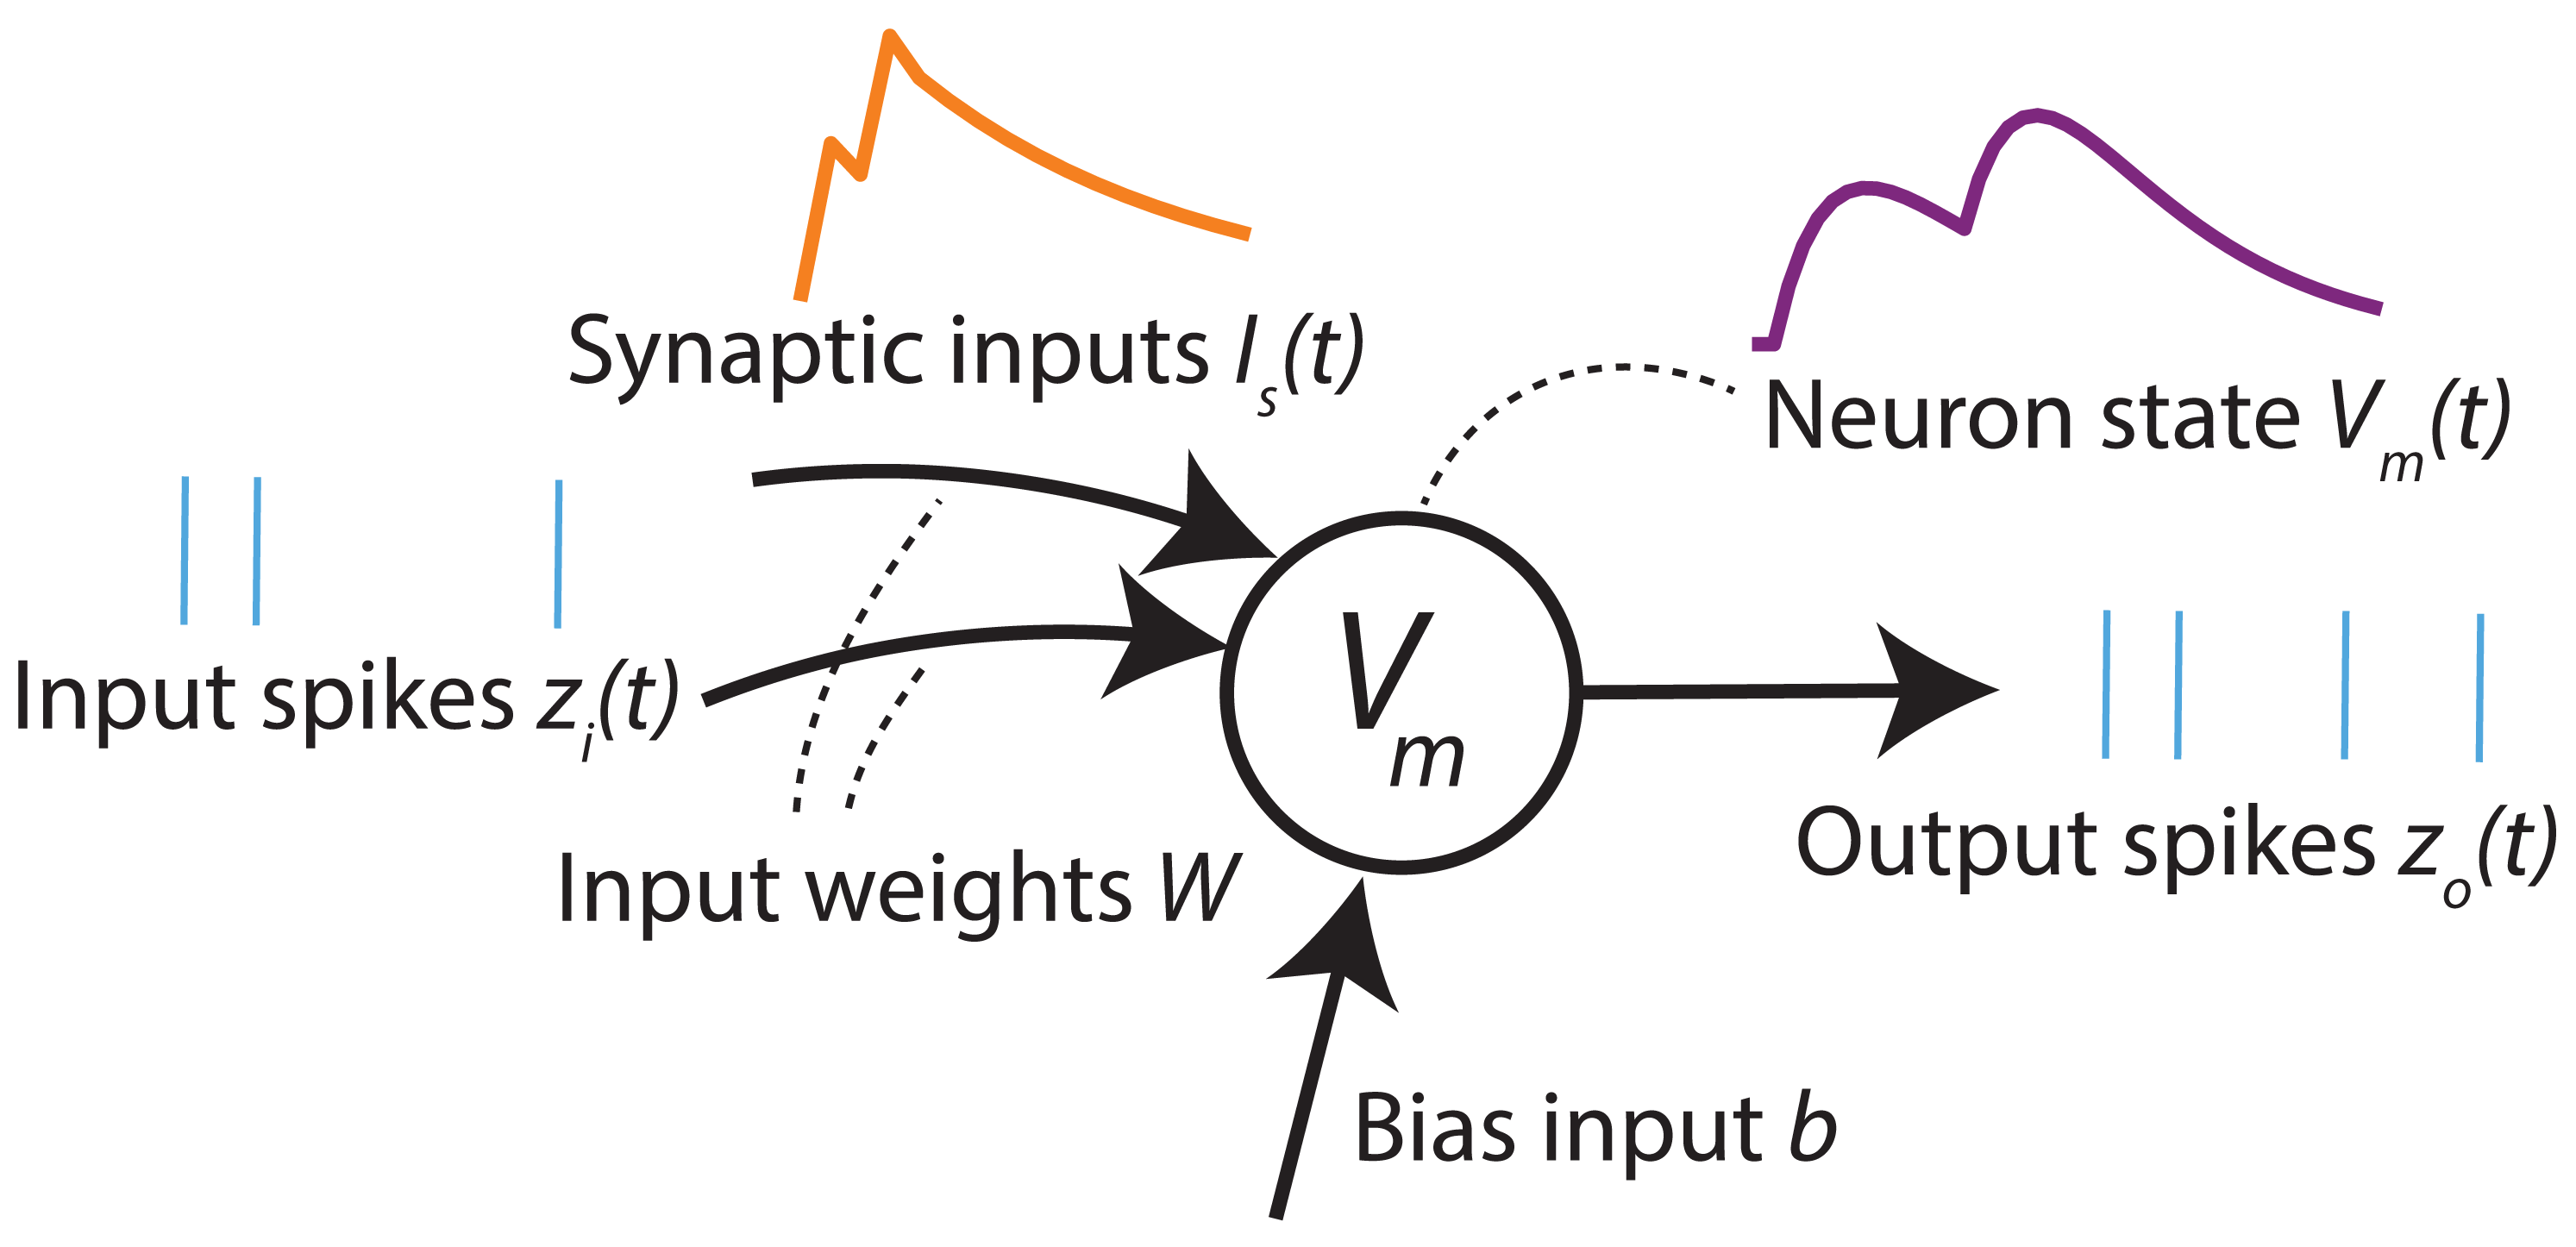
\includegraphics[width=0.9\colwidth]{LIF.png} \\
\vspace{1em}
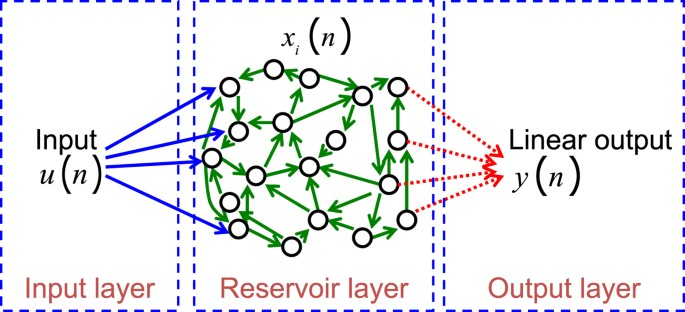
\includegraphics[width=0.9\colwidth]{LSM.jpg}
\end{block}

\end{column}
\separatorcolumn

\begin{column}{\colwidth}

\begin{block}{How have others implemented and/or accelerated this algorithm?}
Spiking neural networks and LSMs have been implemented in digital hardware (e.g., FPGAs, GPUs, and neuromorphic platforms such as Intel's Loihi). Most software implementations (e.g., \texttt{snntorch}, Brian2, NEST) emulate spiking dynamics using clocked digital logic. 
\end{block}


\begin{block}{What are you doing differently?}
Unlike clocked digital models, this implementation runs in continuous time and may enable a better approximation to biological dynamics. The analog nature also opens the door for ultra-low power neuromorphic inference systems.
\end{block}

\begin{block}{Discrete VS Continuous Time}
\centering
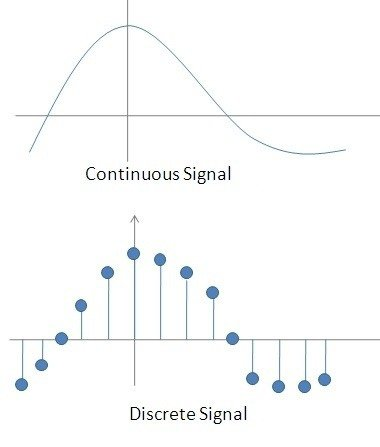
\includegraphics[width=0.9\colwidth]{time.jpg} \\
\end{block}

\end{column}
\separatorcolumn

\begin{column}{\colwidth}

\begin{block}{What have you accomplished so far?}
\begin{itemize}
  \item Designed and simulated a working LIF neuron circuit in SPICE.
  \item Verified leaky integration and reset behavior under constant current input.
  \item Generated a digital spike output (\texttt{spike\_out}) when membrane voltage exceeds a threshold.
\end{itemize}
\end{block}


\begin{block}{What will you do next?}
\begin{itemize}
  \item Expand to a multi-neuron reservoir with interconnections.
  \item Add synaptic connectivity (resistive or capacitive).
  \item Record spike trains and train a software-based readout layer (e.g., logistic regression) on benchmark time-series tasks.
  \item Quantify energy per spike and compare with digital baselines.
  \item Explore scaling and layout feasibility toward an analog ASIC.
\end{itemize}
\end{block}

\end{column}

\separatorcolumn

\end{columns}

\end{frame}
\end{document}

